% !TEX encoding = UTF-8 Unicode
\documentclass{article}
%\documentclass[12pt,reqno]{amsart}
\usepackage[russian]{babel}
\usepackage[utf8]{inputenc}
%\usepackage[dvips]{graphicx,graphics}
\usepackage{graphicx}
\usepackage{euscript}
\usepackage{graphics}
%\usepackage{russcorr}
\usepackage[active]{srcltx} % SRC Specials: DVI [Inverse] Search
\usepackage{amssymb,amsmath,amsthm,amsfonts}
\usepackage{amsopn}
\newtheorem{cor}{Следствие}
\newtheorem{lem}{Лемма}
\newtheorem{thm}{Теорема}
\newtheorem{prop}{Предложение}
\newtheorem*{thm_pres}{Теорема}
\theoremstyle{definition}
\newtheorem{defn}{Определение}
\newtheorem{defneq}{Эквивалентное определение}
\theoremstyle{remark}
\newtheorem*{rem}{Замечание}
\newtheorem*{deff}{Обозначение}
\usepackage{verbatim}
\usepackage{listings}
\usepackage{hyperref}
\usepackage{color}

\definecolor{dkgreen}{rgb}{0,0.6,0}
\definecolor{gray}{rgb}{0.5,0.5,0.5}
\definecolor{mauve}{rgb}{0.58,0,0.82}

\lstset{frame=tb,
  language=Java,
  aboveskip=3mm,
  belowskip=3mm,
  showstringspaces=false,
  columns=flexible,
  basicstyle={\small\ttfamily},
  numbers=none,
  numberstyle=\tiny\color{gray},
  keywordstyle=\color{blue},
  commentstyle=\color{dkgreen},
  stringstyle=\color{mauve},
  breaklines=true,
  breakatwhitespace=true,
  tabsize=3
}

\newcommand{\sug}[1]{\rule[-2mm]{0.4pt}{5mm}_{\,{#1}}}
\newcommand{\gen} {$GE^+_n(\mathbf{R}[x])\ $}
\newcommand{\genn} {$GE^+_2(\mathbf{R}[x])\ $}
\newcommand{\gn} {$G_n(\mathbf{R})\ $}
\newcommand{\gln} {$GL_n(\mathbf{R}[x])\ $}
\newcommand{\p} {\mathbf{P}}
\newcommand{\peq} {$\mathcal{P}$}
\newcommand{\po} {$\mathcal{P}_0$}
\newcommand{\ff} {$\mathbf{R}\ $}
\newcommand{\fx} {\mathbf{R}[x]}
\newcommand{\fp} {\mathbf{R_+}}
\newcommand{\fxp} {\mathbf{R_+}[x]}
\newcommand{\zx} {\mathbb{Z}[x]}
\newcommand{\zxp} {\mathbb{Z_+}[x]}
\newcommand{\basering} {$\mathbf{F}$}
\newcommand{\lfrac} [2] {\displaystyle \frac{#1}{#2}}
\newcommand{\brsum} [3] {\displaystyle \sum \limits_{#1}^{#2} \left( #3\right)}
\newcommand{\lsum} [2] {\displaystyle \sum \limits_{#1}^{#2}}
\newcommand{\br} [1] {\left( #1 \right)}
\newcommand{\tab} {\mbox{             } \quad }
\usepackage{a4wide}

\usepackage{verbatim}
\usepackage{hyperref}
\hypersetup{
    colorlinks,
    citecolor=black,
    filecolor=black,
    linkcolor=blue,
    urlcolor=blue
}
\setcounter{secnumdepth}{0}


\renewcommand*\contentsname{Summary}

\begin{document}

\begin{center}
\Large{\bf Финальный отчет по проекту ``Рекламный сервер''.}
\end{center}

\tableofcontents

\newpage

\section{Структура проекта.}

Проект ``Рекламный Сервер'' реализован с помощью двух языков программирования -- С++ и Python. С++ые исходники с численными методами динамически импортятся в код интерфейса написаного на питоне. Для написания интерфейса использоватся flask-фреймфорк.


\subsection{Схема проекта}



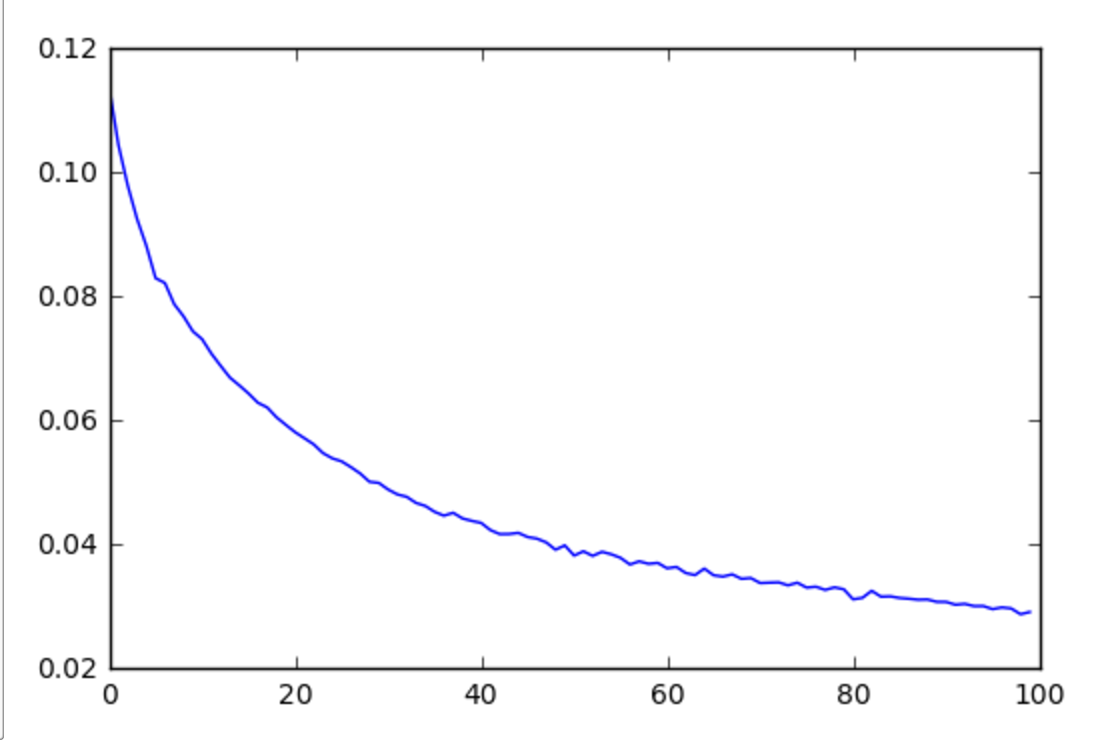
\includegraphics[width=1 \textwidth]{1.png}

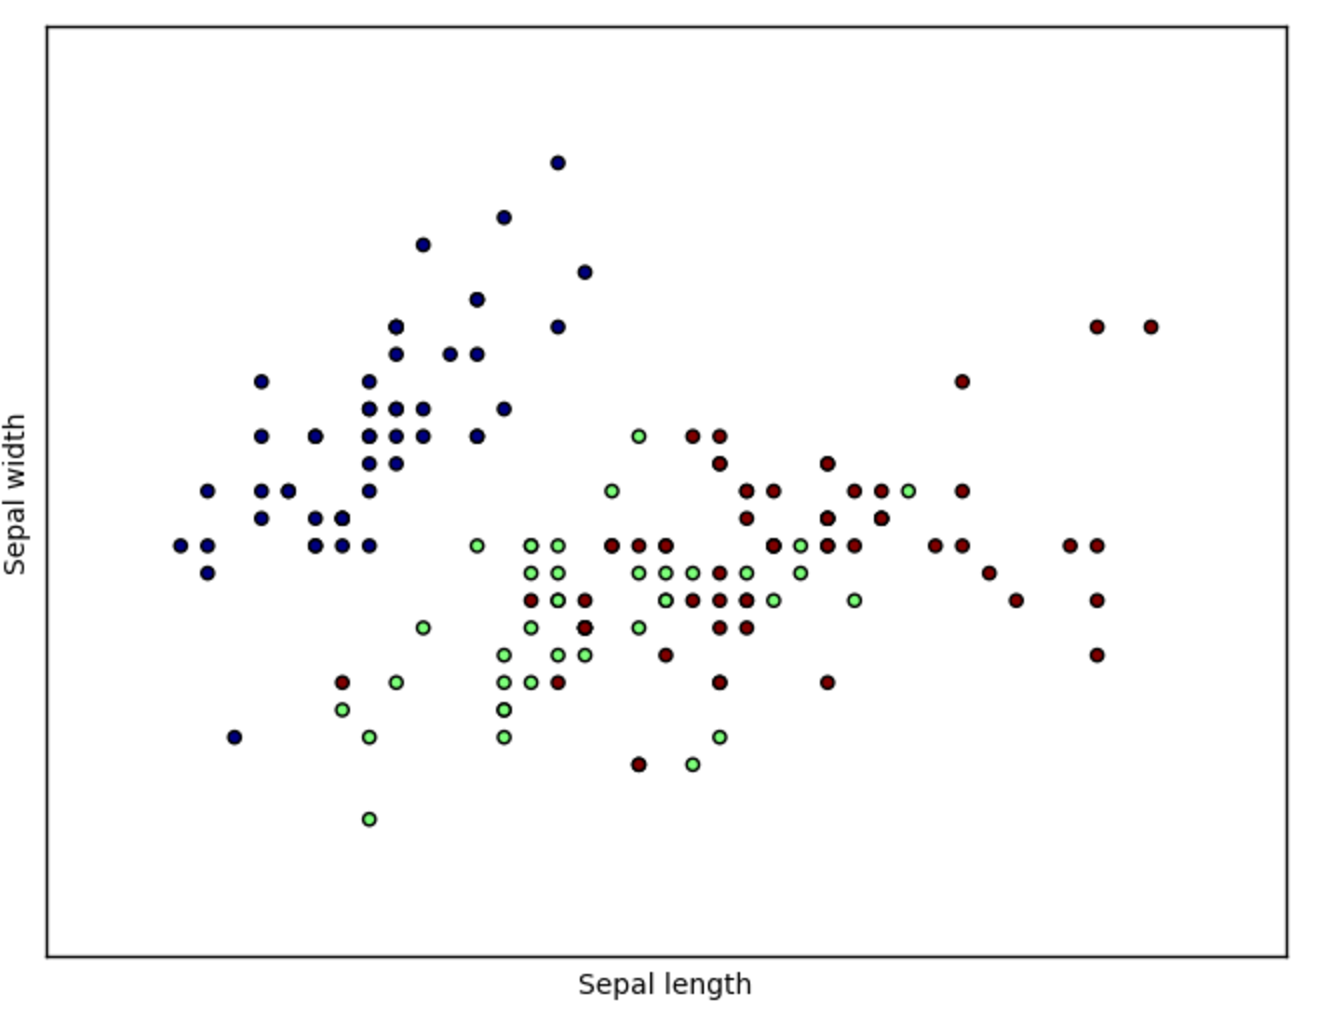
\includegraphics[width=1 \textwidth]{2.png}


\subsection{Сигнатуры функций}
В рамках проекта были реализованы следующий модули и классы:


$\bullet$ класс TabularFunction -- класс табулированной функции -- хранит в себе мап x->y.


Подкласс TabularFunctionConstIterator -- итератор по хранящимся значениям.


Функции:

Дефолтный конструктор
\begin{lstlisting}
	TabularFunction();
\end{lstlisting}


Конструктор копирования

\begin{lstlisting}
	TabularFunction(const TabularFunction& function);
\end{lstlisting}

Функция получения всех известных значений данной функции

\begin{lstlisting}
	std::map<double, double> GetValues() const;
\end{lstlisting}

Функция получения значения функции по значению аргумента

\begin{lstlisting}
	double GetValue(const double argument) const;
\end{lstlisting}


Функция добавления нового значения

\begin{lstlisting}
	void AddValue(const double argument, const double value);
\end{lstlisting}


Функция получения итератора на начало мапа со значениями

\begin{lstlisting}
	TabularFunctionConstIterator Begin() const;
\end{lstlisting}


Функция получения количества известных значений функции
\begin{lstlisting}
	size_t Size() const;
\end{lstlisting}


Функция дифференцирования табулированной функции

\begin{lstlisting}
	TabularFunction Diff() const;
\end{lstlisting}

Функция умножения значений данной функции на какое то число

\begin{lstlisting}
	TabularFunction MultiplyBy(const double value) const;
\end{lstlisting}


Функция смещения значения данной функции в 0 в указаной точке точке
\begin{lstlisting}
	TabularFunction MakeValueZero(const double zero_arg) const;
\end{lstlisting}

Функция уснозения значений данной функции на значения аргумента
\begin{lstlisting}
	TabularFunction MultiplyByArgument() const;
\end{lstlisting}


Функция преобразования f(x) в f(y(x))
\begin{lstlisting}
	TabularFunction Combine(const TabularFunction& inner) const;
\end{lstlisting}

Функция домножения данной функции на другую
\begin{lstlisting}
	TabularFunction MultiplyByAnotherFunction(const TabularFunction& another_function) const;
\end{lstlisting}

Функция вывода на экран всех известных значений данной функции
\begin{lstlisting}
	void Print() const;
\end{lstlisting}


$\bullet$ класс TabulateIntegration -- модуль позволяющий вычислять интеграл табулированной функции методом трапеций.

Функция вычисления интеграла табулированной функции
\begin{lstlisting}
	TabularFunction Integrate(const TabularFunction& function) const;
\end{lstlisting}

$\bullet$ класс LinearSystemSolution -- класс решения линейной системы алгебраических уравнений.


Подкласс ConstIterator итератор по полученным значениям x

Функции:

Функция получения итератора на начало ответов

\begin{lstlisting}
	ConstIterator begin() const;
\end{lstlisting}

Функция получения итератора на конец ответов

\begin{lstlisting}
	ConstIterator end() const;
\end{lstlisting}

Конструктор

\begin{lstlisting}
	LinearSystemSolution(const std::vector<double>& solution);
\end{lstlisting}

Функция для определения наличия ответа в данном классе

\begin{lstlisting}
	bool IsThereSolution() const;
\end{lstlisting}

Функция получения вектора ответов из данного класса
\begin{lstlisting}
	std::vector<double> GetSolution() const;
\end{lstlisting}

$\bullet$ класс LinearSystem -- класс вычисления решения линейной системы алгебраических уравнений.

Функции:

Функция очищения системы

\begin{lstlisting}
	LinearSystem& clear();
\end{lstlisting}

Функция добавления линейного уравнения в систему

\begin{lstlisting}
	LinearSystem& AddEquation(const std::vector<double>& new_left_part, const double right_part);
\end{lstlisting}

Функция свапа двух уравнений в системе
\begin{lstlisting}
	LinearSystem& SwapEquations(const size_t first_index, const size_t second_index);
\end{lstlisting}

Функция деления коэффициентов данного уравнения из системы на какое то число
\begin{lstlisting}
	LinearSystem& Transformation(const size_t first_index, const size_t second_index, const double coefficient);
\end{lstlisting}

Функция решения системы уравнений
\begin{lstlisting}
	LinearSystemSolution Solve();
\end{lstlisting}

$\bullet$ класс CubeSpline -- класс кубического сплайна.

Функции:

Конструктор

\begin{lstlisting}
	CubeSpline(const double a, const double b, const double c, const double d, const double x)
\end{lstlisting}

Функция получения значения сплайна в данной точке
\begin{lstlisting}
	double GetValue(const double x) const;
\end{lstlisting}


$\bullet$ класс Interpolator.

Функции:

Конструктор

\begin{lstlisting}
	Interpolator(const TabularFunction& function);
\end{lstlisting}

Функция получения значения интерполированной функции по аргументу

\begin{lstlisting}
	double GetValue(const double x) const;
\end{lstlisting}

Функция получения табулированной функции из интерполированной

\begin{lstlisting}
	TabularFunction GetTabularFunction(const double precise_step) const;
\end{lstlisting}

$\bullet$ класс CauchySolution --  класс решения задачи Коши -- две табулированные функции от t.

Функции:

Функция получения значений первой функции

\begin{lstlisting}
	TabularFunction GetX() const;
\end{lstlisting}

Функция получения значений второй функции

\begin{lstlisting}
	TabularFunction GetY() const;

\end{lstlisting}

$\bullet$ класс BaseCauchyFunction -- базовый класс для функции из задачи Коши.


$\bullet$ класс CircleCauchyFunction -- функция для которой решения задачи Коши -- круг.

Функции:

Функция получения значения X
\begin{lstlisting}
	double GetValueX(const double x, const double y, const double t) const;
\end{lstlisting}


Функция получения значения Y

\begin{lstlisting}
	double GetValueY(const double x, const double y, const double t) const;
\end{lstlisting}

$\bullet$ класс SpiralCauchyFunction -- функция для которой решения задачи Коши -- спираль.

Функции:

Функция получения значения X
\begin{lstlisting}
	double GetValueX(const double x, const double y, const double t) const;
\end{lstlisting}


Функция получения значения Y

\begin{lstlisting}
	double GetValueY(const double x, const double y, const double t) const;
\end{lstlisting}


$\bullet$ класс CauchyProblem -- модуль для решения задачи Коши методом Эйлера.

Функции:

Конструктор принимающий ограничения на значения аргументов и векторфункцию f.

\begin{lstlisting}
	CauchyProblem(const double x0, const double y0, const double x_min, const double x_max, const double y_min, const double y_max, const double t_min, const double t_max, const double t_step, BaseCauchyFunction * f);
\end{lstlisting}

$\bullet$ класс ParametrisedAdBaseFunction -- базовый класс функции f.

Функции:

Функция присваивания значения бете

\begin{lstlisting}
	virtual void SetBeta(const double new_beta);

\end{lstlisting}

Функция получения значения беты

\begin{lstlisting}
	virtual double GetBeta() const;

\end{lstlisting}

Функция получения значения данной функции

\begin{lstlisting}
	virtual double GetValue(const double z, const double x, const double S) const;

\end{lstlisting}

$\bullet$ класс SimpleDiffAdFunction -- beta * (S - x).


$\bullet$ класс AdCauchyFunction -- функция для задачи коши соответствующая ParametrisedAdBaseFunction.

Функции:

Конструктор

\begin{lstlisting}
	AdCauchyFunction(const Interpolator& z_diff, const Interpolator& U, const Interpolator& z, const Interpolator& S, ParametrisedAdBaseFunction* f_beta);
\end{lstlisting}

Функция получения значения беты из

\begin{lstlisting}
	f_beta double GetBeta() const;
\end{lstlisting}

Функция получения значения X (первой функции z\_diff.GetValue(t) * U.GetValue(y))

\begin{lstlisting}
	double GetValueX(const double x, const double y, const double t) const;
\end{lstlisting}

Функция поучения занчения(f\_beta->GetValue(z.GetValue(t), x, S.GetValue(t))) Y

\begin{lstlisting}
	double GetValueY(const double x, const double y, const double t) const;
\end{lstlisting}

Функция записи беты

\begin{lstlisting}
	void SetBeta(const double beta);
\end{lstlisting}

$\bullet$ класс AdServer -- базовый класс сервера являющийся интерфейсом для ручного режима.

Функции:

Конструктор

\begin{lstlisting}
	AdServer(const TabularFunction& rho, const TabularFunction& S, ParametrisedAdBaseFunction * f_beta, const TabularFunction& z, const double x0, const double y0, const double T, const double step)
\end{lstlisting}


Сеттеры

\begin{lstlisting}
	void SetBeta(const double beta); void SetX0(const double x0); void SetY0(const double y0);
\end{lstlisting}

Геттеры полученных значений функций

\begin{lstlisting}
	TabularFunction GetS() const; TabularFunction GetX() const; TabularFunction GetY() const; double GetBeta() const;
\end{lstlisting}

Функция для решения задачи Коши относительно z.Diff(), Interpolator(integration.Integrate(rho).MultiplyBy(-1).MakeValueZero(1.)), Interpolator(z), Interpolator(S), f\_beta

\begin{lstlisting}
	void SolveCauchyProblem();

\end{lstlisting}


Функции для получения значений функционалов качества

\begin{lstlisting}
	double C1() const;
	double C2() const;
	double Phi() const;

\end{lstlisting}



$\bullet$ класс AdServerAutoSetup --  базовый класс сервера являющийся интерфейсом для автоматического режима.

Функции:

Конструктор

\begin{lstlisting}
	AdServerAutoSetup(const AdServer& ad_server, const double beta_min, const double beta_max, const double beta_precision);
\end{lstlisting}

Сеттеры

\begin{lstlisting}
	void SetX0(const double x0); void SetY0(const double y0);

\end{lstlisting}

Функция поиска оптимального значения ветта с помощью тернарного поиска

\begin{lstlisting}
	void SetupOptimalBeta();
\end{lstlisting}

Геттер сервера который делает вычисления все функционалов при заданной бете

\begin{lstlisting}
	AdServer GetAdServer() const;
\end{lstlisting}




\section{Метод трапеций}

\subsection{Простая и составная формула метода трапеций}

Простая формула метода трапеций:

$$
\int \limits_{a}^{b} f(x) dx \approx \lfrac{f(a) + f(b)}{2}(b - a)
$$

Составная формула метода трапеций:

$$
\int \limits_{a}^{b} f(x) dx \approx \sum \limits_{i = 0}^{n - 1} \left( \lfrac{f(x_i) + f(x_{i + 1})}{2} (x_{i + 1} - x_i)\right)
$$

\subsection{Оценка аналитического порядка точности}

Рассмотрим функцию f на отрезке от $x_i$ до $x_i + h$. Разложим ее в ряд Тейлора с остаточным членом в форме Лагранжа

$$
f(x) = f(x_i) + (x - x_i) f^\prime(x_i) + \lfrac{(x - x_i)^2}{2}f^{\prime\prime}(\xi),
$$

где $\xi \in [x_i, x_i + h]$.

Проинтегрируем это разложение:

$$
\int\limits_{x_i}^{x_i + h} f(x) dx = h  f(x_i) + \lfrac{h^2}{2} f^\prime(x_i) + \lfrac{h^3}{6} f^{\prime\prime}(\xi).
$$

Также подставим $x = x_i + h$ в это разложение

$$
f(x_i + h) = f(x_i) + h f^{\prime}(x_i) + \lfrac{h^2}{2}f^{\prime\prime}(\xi).
$$

Преобразуем последние два соотношения: вычтем из первого второе, домноженое на $h/2$:

$$
\int\limits_{x_i}^{x_i + h} f(x) dx - \lfrac{h}{2} f(x_i + h) = \lfrac{h}{2} f(x_i)  - \lfrac{h^3}{12} f^{\prime\prime}(\xi).
$$

$$
\left| \int\limits_{x_i}^{x_i + h} f(x) dx - \lfrac{f(x_{i + 1}) - f(x_i)}{2}(x_{i + 1} - x_i)\right| \leq ||f^{\prime\prime}||\lfrac{h^3}{12}
$$

Просуммировав эти неравенства по всем отрезкам $[x_i, x_{i + 1}]$ получим, что общий уровень ошибки меньше, чем

$$
||f^{\prime\prime}||\lfrac{h^3}{12} * \lfrac{b-a}{h} = ||f^{\prime\prime}||\lfrac{h^2(b - a)}{12}.
$$

Это означает, что порядок точности второй.

\subsection{Реализация на sage для последующих оценок метода}

\begin{lstlisting}
def get_segments(a, b, step):
        x = a
        while (x + step <= b):
                yield (x, x + step)
                x += step

def trapesoid_integrate(func, a, b, step):
        integral = 0
        for (x, y) in get_segments(a, b, step):
                integral += (func(x) + func(y)) / 2 * (y - x)

        return integral
\end{lstlisting}

\subsection{Сравнение методов с встроенными методами sage для примеров}

Сравнивающий код:

\begin{lstlisting}
from sage.symbolic.integration.integral import definite_integral

for (func, a, b) in (
	(x^3, 1, 2),
	(sgn(x), -1, 1),
	(sin(1/x), 0.000001, 1),
):
	print "Func {func} on segment [{a}, {b}]: trapesoid method value : {trapesoid_value}, real value : {real_value}".format(
		func=func, a=a, b=b, trapesoid_value = trapesoid_integrate(func,a, b, 0.001), real_value = float(definite_integral(func, x, a, b))
	)
\end{lstlisting}

Вывод кода:

\begin{lstlisting}
Func x^3 on segment [1, 2]: trapesoid method value : 3.75000074999912, real value : 3.75
Func sgn(x) on segment [-1, 1]: trapesoid method value : -5.55111512312578e-17, real value : 0.0
Func sin(1/x) on segment [1.00000000000000e-6, 1]: trapesoid method value : 0.500258204182386, real value : 0.504067061906
\end{lstlisting}

Видно, что для гладкой и разрывной функции удалось довольно хорошо вычислить значение интеграла. С осциллирующей функцией получилось не так хорошо, есть ошибка уже в тысячных долях. Это произошло, потому что ее значение второй производной велико.

\subsection{Экспериментальный анализ точности метода}


Код для анализа:

\begin{lstlisting}
func = x^4
a = 1.
b = 2.
points = []
for segments_count in xrange(2, 500):
	step = (b - a) / segments_count
	error = abs(float(definite_integral(func, x, a, b)) - trapesoid_integrate(func, a, b, step))
	points.append((log(segments_count), log(error)))
line(points)
\end{lstlisting}

Полученный график

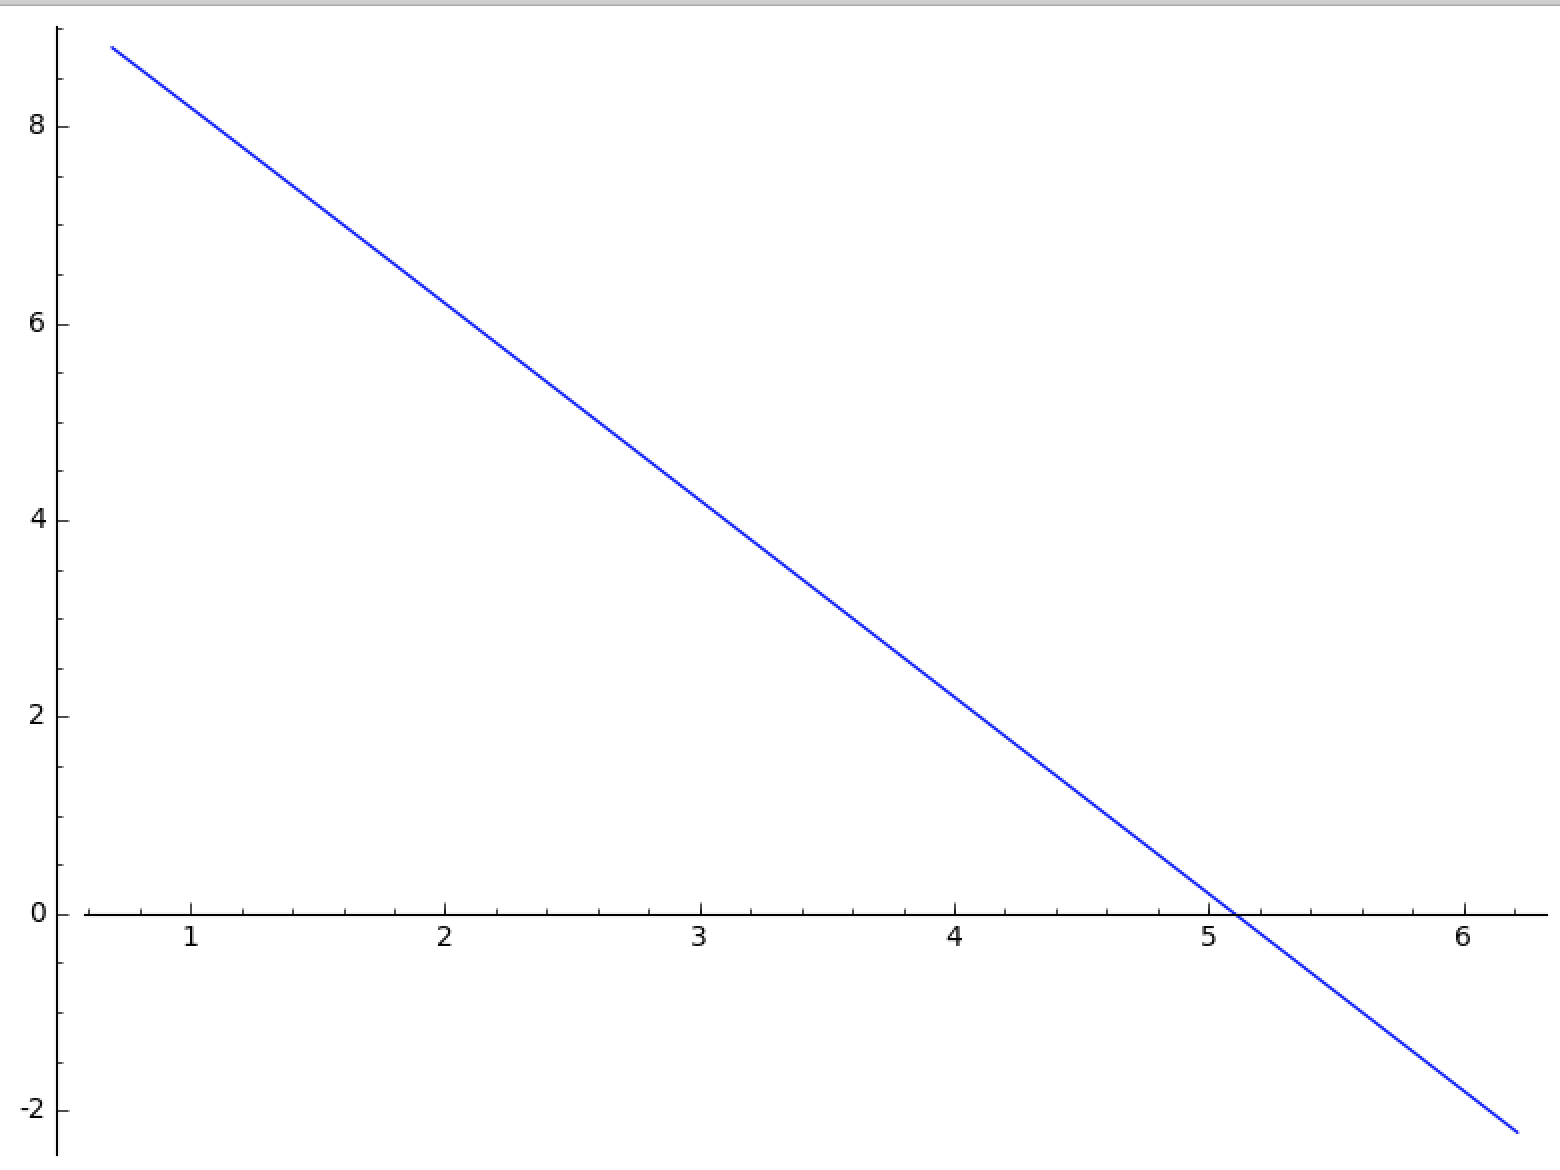
\includegraphics[width=0.9 \textwidth]{image.png}

На нем видим, что изначально, когда сегментов мало, ошибка большая, а потом она уменьшается и логарифм ошибки уже становится отрицательным. Наклон кривой как раз равен $-2$, что подтверждает теоретические заключения о втором порядке погрешности.


\section{Метод Гаусса}

\subsection{Описание метода Гаусса решения системы линейных уравнений}
Метод Гаусса заключается в том, что сначала нужно выписать матрицу линейной системы уравнений и столбец свободных коэффициентов справа от нее. Далее, нужно совершать элементарные преобразования строк с матрицей и такие же преобразования строк со столбцом свободных коэффициентов (элементарное преобразование -- это вычитание из одной строки другой строки, домноженной на любой коэффициент).

Метод работает тогда и только тогда, когда определитель матрицы уравнения отличен от нуля. Пусть это так. Тогда в первом столбце матрицы есть ненулевое число. Перенесем строку с этим числом на первое место, а затем из всех остальных строк, начиная со второй, вычтем первую строку с таким коэффициентом, чтобы все элементы в первом столбце, кроме первого, стали равны нулю. Далее рассмотрим подматрицу исходной матрицы, начиная со второй строки и второго столбца и применим к ней тот же алгоритм.

В итоге, матрица будет иметь верхнетреугольный вид с ненулевыми коэффициентами на диагонали. После этого, наоборот, вычитаем из всех строк последнюю с таким коэффициентом, чтобы занулить все числа в последнем столбце кроме последнего. Затем, рассматриваем подматрицу исходной матрицы без последнего столбца и последней строки и применяем к ней тот же алгоритм.

В итоге, матрица будет иметь диагональный вид. Остается лишь решить систему уравнений, в которой уравнения имеют вид $k_i x_i = b_i$, и решение будет иметь вид $x_i = \lfrac{b_i}{k_i}$.

\subsection{Обоснование корректности метода Гаусса решения системы линейных уравнений}

Метод Гаусса использует элементарные преобразования строк матрицы и корректен, потому что соблюдение условий $f = 0, g = 0$ равносильно соблюдению условий $f + \lambda g = 0, g = 0$.

Система уравнений преобразуется к равносильной ей системе, которая затем решается.

\subsection{Условия применимости метода Гаусса для решения линейной системы уравнений}

Как уже было сказано ранее, для конструкции необходимо, чтобы определитель матрицы был отличен от нуля, иначе на очередном шаге мы не можем гарантировать, что найдем ненулевой элемент для того, чтобы за его счет обнулить все остальные в столбце.

\subsection{Вычисления с тремя матрицами}

Для вычисления определителей, матричных норм и неувязок используем sage

Код программы:

%http://www.cyberforum.ru/cpp-beginners/thread102517.html
%https://ru.wikipedia.org/wiki/Число_обусловленности
\begin{lstlisting}
def get_modules_sum(numbers):
	return sum(abs(x) for x in numbers)

def get_line_modules_sum(cur_matrix):
	for line in cur_matrix:
		yield get_modules_sum(line)

def get_infty_norm(cur_matrix):
	return max(get_line_modules_sum(cur_matrix))

def get_conditionality_number(cur_matrix):
	return get_infty_norm(cur_matrix) * get_infty_norm(cur_matrix^(-1))

def elementary_transformation(cur_matrix, coefs, i, j, la):
	cur_matrix[i] -= cur_matrix[j] * float(la)
	coefs[i] -= coefs[j] * float(la)

def swap_rows(cur_matrix, coefs, i, j):
	(cur_matrix[i], cur_matrix[j]) = (cur_matrix[j], cur_matrix[i])
	(coefs[i], coefs[j]) = (coefs[j], coefs[i])

def gauss_solve(cur_matrix, coefs):
	for start_row_index in xrange(cur_matrix.nrows()):
		max_row_index = None
		max_col_value = None
		for row_index in xrange(start_row_index, cur_matrix.nrows()):
			if max_col_value == None or max_col_value < abs(cur_matrix[row_index][start_row_index]):
				max_col_value = abs(cur_matrix[row_index][start_row_index])
				max_row_index = row_index

		swap_rows(cur_matrix, coefs, start_row_index, max_row_index)

		for row_index in xrange(start_row_index + 1, cur_matrix.nrows()):
			elementary_transformation(
				cur_matrix,
				coefs,
				row_index,
				start_row_index,
				cur_matrix[row_index][start_row_index]
					/ cur_matrix[start_row_index][start_row_index]
			)

	for start_row_index in xrange(cur_matrix.nrows() - 1, -1, -1):
		for row_index in xrange(start_row_index - 1, -1, -1):
			elementary_transformation(
				cur_matrix,
				coefs,
				row_index,
				start_row_index,
				cur_matrix[row_index][start_row_index]
					/ cur_matrix[start_row_index][start_row_index]
			)

	for row_index in xrange(cur_matrix.nrows()):
		yield coefs[row_index] / cur_matrix[row_index][row_index]

def make_column(vector):
	return matrix([[x] for x in vector])

def calc_error_vector(cur_matrix, coefs, solution):
	return make_column(coefs) - cur_matrix * make_column(solution)

def calc_error(cur_matrix, coefs, solution):
	return max(line[0] for line in calc_error_vector(cur_matrix, coefs, solution))

A = matrix([[1,2,3],[2.0001,3.999,6],[15,3,6]])
B = matrix(QQ, 8, 8, lambda i, j: 1./(i + j + 1))
C = matrix([[float(10^6),float(2)],[float(10^13),float(2)]])

rows = [["det","matrix_norm","conditionality_number","error"]]
for cur_matrix in (A, B, C):
	infty_norm = get_infty_norm(cur_matrix)
	conditionality_number = get_conditionality_number(cur_matrix)
	b = list(1 for i in xrange(cur_matrix.nrows()))
	solution = list(gauss_solve(cur_matrix, b))
	error = calc_error(cur_matrix, b, solution)
	rows.append([
		float(det(cur_matrix)),
		float(infty_norm),
		float(conditionality_number),
		error,
	])
print table(rows)
\end{lstlisting}

Вывод программы:

\begin{lstlisting}
  det                 matrix_norm     conditionality_number   error
  -0.0387             24.0            72557.9534884           0.0
  2.73705011549e-33   2.71785714286   33872791095.0           9.04844199567e-09
  1.9999998e+13       1e+13           5.000001e+12            0.0
\end{lstlisting}

Вывод: точный метод Гаусса ошибается при большом числе обусловленности, а при большой норме -- не обязательно.

\section{Интерполяция кубическими сплайнами}

\subsection{Описание интерполяции кубическими сплайнами}

Дан отрезок, разбитый на много маленьких отрезков. Даны значения некоторой неизвестной функции в узлах сетки. В алгоритме аппроксимации, на каждом маленьком отрезочке мы пытаемся найти кубическую функцию, которая совпадает с исходной функцией в точках сетки, при этом добавляем условия равенства первой и второй производной соседних сплайнов в точке сетки, а также добавляем условия на то, что вторая производная в концах отрезка равна нулю.

Все условия являются линейными относительно коэффициентов всех сплайнов, поэтому формируют систему линейных уравнений, которую можно решить, и получить результирующие коэффициенты сплайнов.

\subsection{Вычисления}

В качестве гладкой функции взята $x^3$, в качестве осциллирующей $\sin\left(\lfrac{1}{x}\right)$, а в качестве разрывной -- $\mathrm{sgn}(x)$.

Вот вычисляющий код:

\begin{lstlisting}
def get_segments(a, b, step):
	x = a
	while (x + step <= b):
		yield (x, x + step)
		x += step
	if x < b:
		yield (x, b)

class CubeSpline(object):
	def __init__(self, a, b, c, d, x1):
		self.a = a
		self.b = b
		self.c = c
		self.d = d
		self.x1 = x1

	def get_value(self, x):
		return self.a + self.b * (x - self.x1) + self.c/2 * (x - self.x1)**2 + self.d / 6 * (x - self.x1) ** 3

class SplineConvex(object):
	def __init__(self, func, a, b, step):
		self.splines = []
		self.segments = list(get_segments(a, b, step))
		n = len(self.segments)

		equations = [
			[1] + [0] * n,
			[0] * n + [1],
		]
		b = [
			0,
			0,
		]

		for i in xrange(1, n):
			(x_i_prev, x_i) = self.segments[i - 1]
			(x_i, x_i_post) = self.segments[i]
			f_i = func(x_i)
			f_i_post = func(x_i_post)
			f_i_prev = func(x_i_prev)
			h_i = x_i - x_i_prev
			h_i_post = x_i_post - x_i
			equations.append(
				[0] * (i - 1) + [h_i, 2 * (h_i + h_i_post), h_i_post] + [0] * (n - i - 1),
			)
			b.append(6 * ((f_i_post - f_i) / h_i_post - (f_i - f_i_prev) / h_i))

		c_coefs = list(gauss_solve(matrix(equations), b))

		for i in xrange(1, n + 1):
			c_i = c_coefs[i]
			c_i_prev = c_coefs[i - 1]
			(x_i_prev, x_i) = self.segments[i - 1]
			f_i = func(x_i)
			f_i_prev = func(x_i_prev)
			h_i = x_i - x_i_prev
			a_i = f_i
			d_i = (c_i - c_i_prev) / h_i
			b_i = (f_i - f_i_prev) / h_i + h_i * (2 * c_i + c_i_prev) / 6
			self.splines.append(CubeSpline(a_i, b_i, c_i, d_i, x_i))


	def get_value(self, x):
		for index in xrange(len(self.segments)):
			(x1, x2) = self.segments[index]
			spline = self.splines[index]
			if x1 <= x and x <= x2:
				return spline.get_value(x)



for (func, a, b, func_name) in (
	(x^3, 1., 2., "x_cubed"),
	(sgn(x), -1., 1., "sign_x"),
	(sin(1/x), 0.000001, 1., "sin_reverse_x"),
):

	g = Graphics()
	g += plot(func, (x, a, b), color='red', legend_label=func_name)
	for (step, color) in ((0.3, 'blue'), (0.05, 'green')):
		spline_convex = SplineConvex(func, a, b, step)
		g += plot(
			lambda t: spline_convex.get_value(t),
			(x, a, b), color=color,
			legend_label="{func_name}_step_{step:.2f}".format(func_name=func_name, step=float(step))
		)

	g.save("{func_name}_splines_image.png".format(func_name=func_name))

	g = Graphics()
	step = 0.05
	spline_convex = SplineConvex(func, a, b, step)
	g += plot(
		lambda t: func(t) - spline_convex.get_value(t),
		(x, a, b), color=color,
		legend_label="{func_name}_interpolation_error".format(func_name=func_name)
	)
	g.save("{func_name}_interpolation_error.png".format(func_name=func_name))
\end{lstlisting}
\newpage

\subsection{Картинки}

Для функции $x^3$

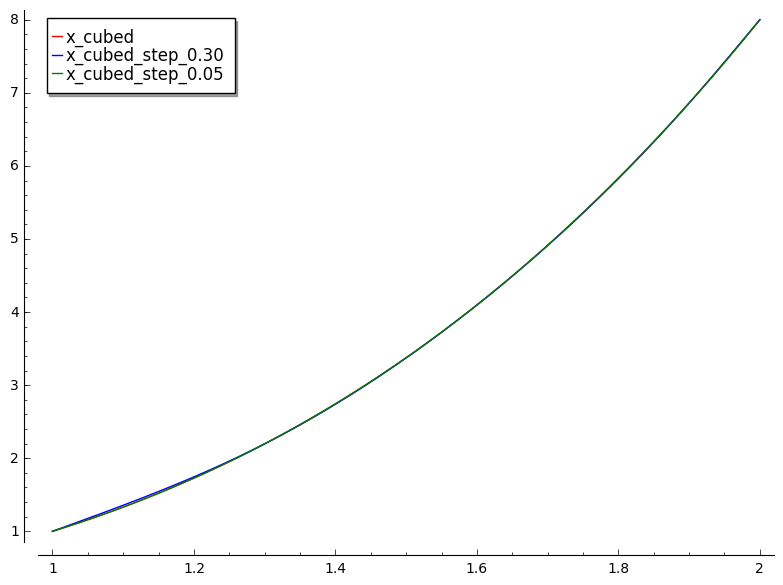
\includegraphics[width=0.4 \textwidth]{x_cubed_splines_image.png}
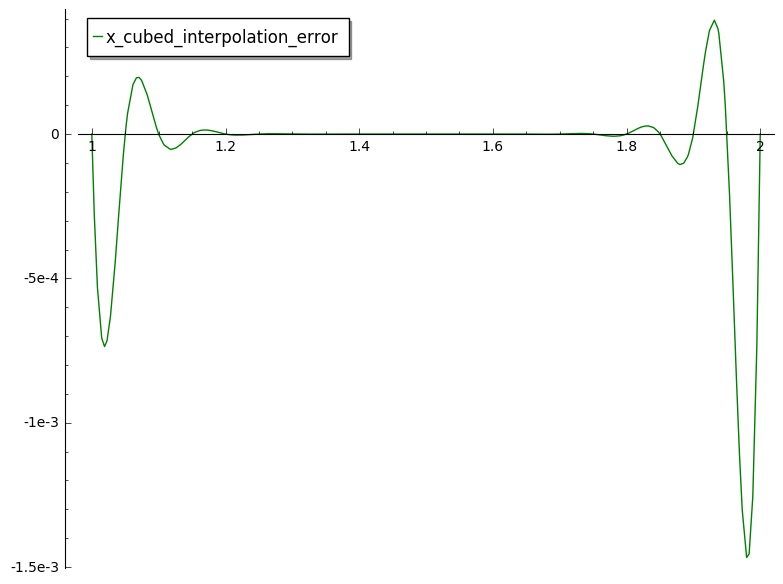
\includegraphics[width=0.4 \textwidth]{x_cubed_interpolation_error.png}

Для функции $\mathrm{sgn}(x)$

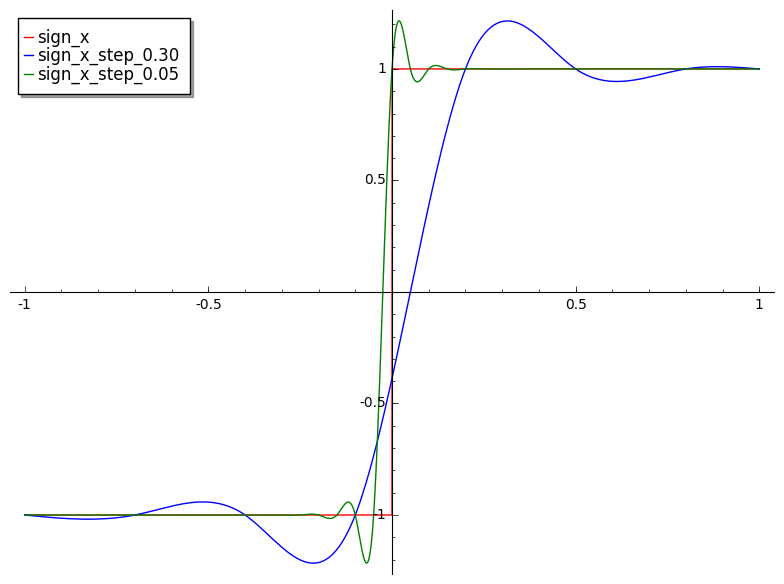
\includegraphics[width=0.4 \textwidth]{sign_x_splines_image.png}
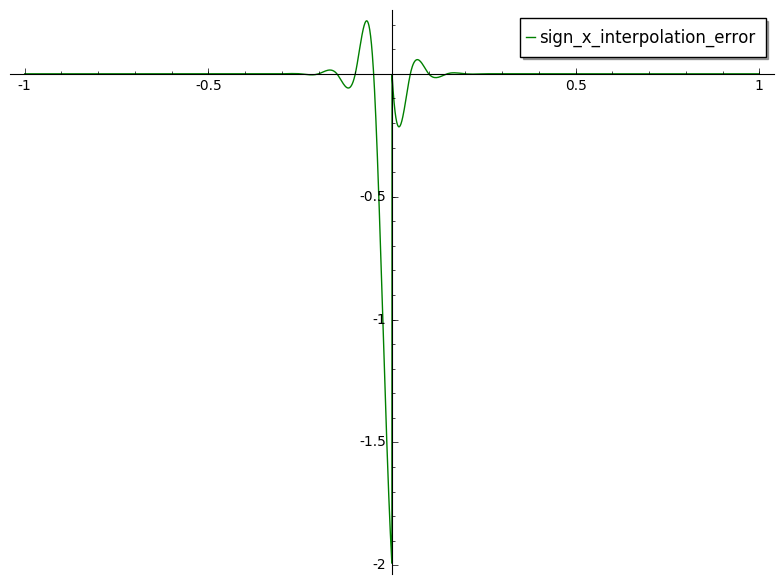
\includegraphics[width=0.4 \textwidth]{sign_x_interpolation_error.png}

Для функции $\sin\left(\lfrac{1}{x}\right)$

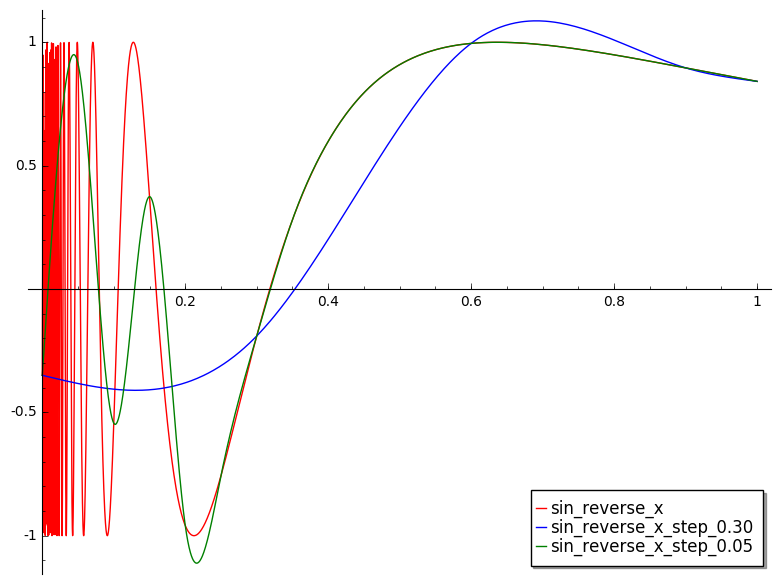
\includegraphics[width=0.4 \textwidth]{sin_reverse_x_splines_image.png}
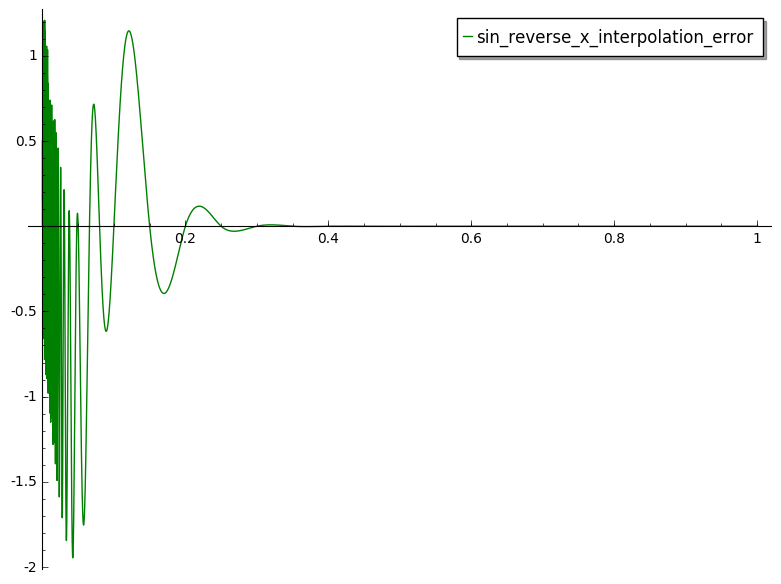
\includegraphics[width=0.4 \textwidth]{sin_reverse_x_interpolation_error.png}

\subsection{Выводы про аппроксимацию}

Гладкую функцию приблизили почти идеально, но на границах приближения есть небольшие артифакты из-за того, что мы приравняли вторую производную на краях нулем, а это в реальной модели не так.

У разрывной функции наблюдаем образование лишних изгибов и экстремумов в районе разрыва.

С оцсиллирующей функцией сплайны справляются очень хорошо до тех пор, пока осцилляции не становятся в несколько раз чаще, чем шаг сетки. Но это логично, тут и невозможно ожидать более хорошего результата.

\section{Решение задачи Коши методом Эйлера}

\subsection{Описание метода решения задачи Коши}

Для решения задачи Коши от двух переменных выбран метод Эйлера. Он заключается в том, что мы строим точки $x_n, y_n, t_n$ по следующему индуктивному правилу:

 $\bullet$ $x_0, y_0$ -- начальная точка из условия задачи Коши, $t_0 = 0$,

 $\bullet$ $x_{n + 1} = x_n + t * f_x(x_n, y_n, t_n),\quad y_{n + 1} = y_n + t * f_y(x_n, y_n, t_n), \quad t_{n+1} = t_n + t$,

где $t$ -- значение временного шага. Чем оно меньше, тем точнее решение, полученное в результате применения метода.

Полученные точки $(x_n, y_n)$ образуют табулированное численное решение.

\subsection{Единственность решения}

Точное решение задачи Коши единственно по теореме о единственности.

Наше численное решение для заданного заранее параметра $t$ также обладает свойством единственности, так как если бы фазовые кривые пересекались, возникло бы противоречие с тем, что для точки пересечения алгоритм построения следующей точки решения детерминирован.

\subsection{Применение решения для конкретной задачи Коши}

Рассмотрим задачу $x^\prime = y,\quad y^\prime = -x, \quad x_0 = 1, \quad y_0 = 0$.

Ее точное решение: $x = cos(t), \quad y = -sin(t)$. Без заданного начального условия, фазовые кривые имеют вид $x = C \mathrm{cos}(t), \quad y = -C \mathrm{sin}(t)$, являются окружностями всех радиусов вокруг начала координат.

Код, строящий графики

\begin{lstlisting}
class DiffEq(object):
	def __init__(self, fx, fy, start_t, end_t, step_t, x0, y0):
		self.fx = fx
		self.fy = fy
		self.start_t = start_t
		self.end_t = end_t
		self.step_t = step_t
		self.x0 = x0
		self.y0 = y0

	def build_solution(self):
		x = []
		y = []
		x_y_data = []
		cur_t = self.start_t
		prev_x = self.x0
		prev_y = self.y0
		prev_t = cur_t
		while cur_t < self.end_t:
			cur_x = prev_x + (cur_t - prev_t) * self.fx(x = prev_x, y = prev_y, t = prev_t)
			cur_y = prev_y + (cur_t - prev_t) * self.fy(x = prev_x, y = prev_y, t = prev_t)
			x.append((cur_t, cur_x))
			y.append((cur_t, cur_y))
			x_y_data.append((cur_x, cur_y))
			prev_x = cur_x
			prev_y = cur_y
			prev_t = cur_t

			cur_t += self.step_t
		self.x = x
		self.y = y
		self.x_y_data = x_y_data


x = var('x')
y = var('y')
t = var('t')
g = Graphics()
g += plot_vector_field((y, -x), (x,-1.1,1.1), (y,-1.1,1.1), color="blue")
g += parametric_plot((cos(t),sin(t)),(t, 0, 2*pi),color="green")
diff_eq = DiffEq(y, -x, 0, 2*pi, 0.01, 1, 0)
diff_eq.build_solution()
g += list_plot(diff_eq.x_y_data, plotjoined=True,color="red")
g.save("diff_eq_solution.png")
\end{lstlisting}
\newpage

Синим цветом обозначено векторное поле, зеленым -- идеальное аналитическое решение, красным -- приближенное решение. Видно, что оно отличается от идеального решения.

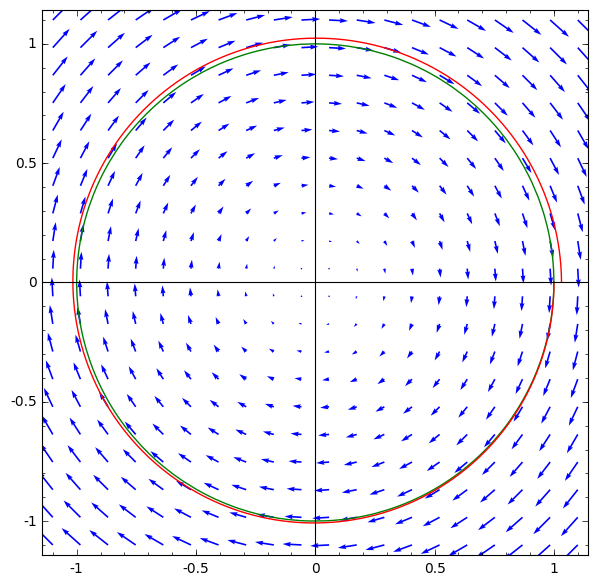
\includegraphics[width=1 \textwidth]{diff_eq_solution.png}

\subsection{Оценка погрешности метода}

Для выше рассмотренной задачи построим графики логарифма ошибки по норме Чебышева от логарифма шага алгоритма.

Код, который строит график ошибки
\begin{lstlisting}
x = var('x')
y = var('y')
t = var('t')
h = 0.3
log_error_points = {}
while h > 0.01:
	diff_eq = DiffEq(y, -x, 0, 2*pi, h, 1, 0)
	diff_eq.build_solution()

	print "for h={h}".format(h=h)
	for (real_func, approx_func, var_name) in ((cos(t), diff_eq.x, 'x'), (-sin(t), diff_eq.y, 'y')):
		max_norm = 0
		cur_t = 0
		for (t_, x_) in approx_func:
			if max_norm < abs(real_func(t_) - x_):
				max_norm = abs(real_func(t_) - x_)

		log_error_points.setdefault(var_name, []).append((-log(h), log(max_norm)))

	h -= 0.01

for var_name in ('x', 'y'):
	g = Graphics()
	g += list_plot(log_error_points[var_name], plotjoined=True, legend_label="{var_name}_error".format(var_name=var_name), gridlines=True)
	g.save("diff_eq_{var_name}_error.png".format(var_name=var_name))
\end{lstlisting}

Графики ошибок:

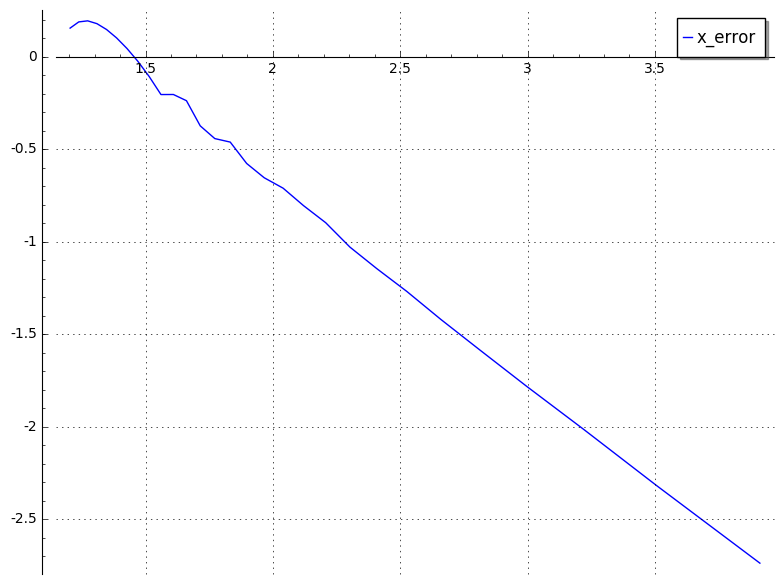
\includegraphics[width=0.4 \textwidth]{diff_eq_x_error.png}
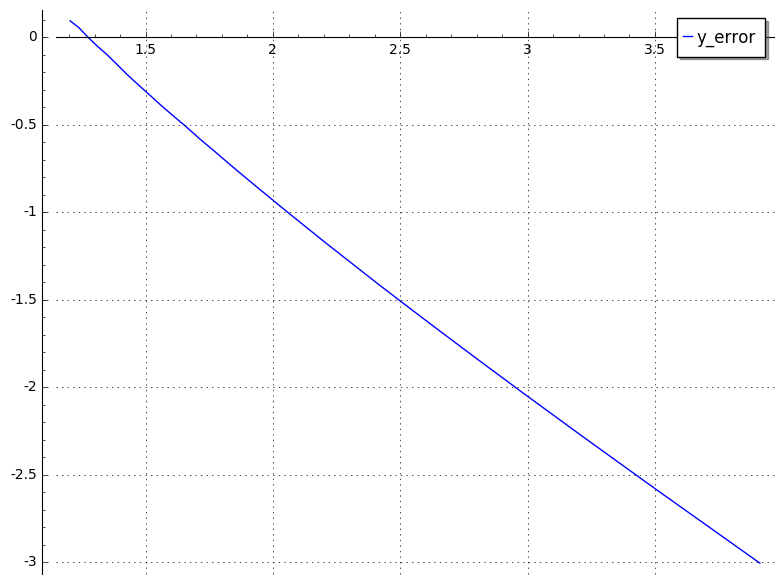
\includegraphics[width=0.4 \textwidth]{diff_eq_y_error.png}

Из них не затруднительно видеть, что метод имеет первый порядок ошибки.



\end{document}
